\documentclass[a4paper]{report}
\usepackage[utf8]{inputenc}
\usepackage[T1]{fontenc}
\usepackage{RJournal}
\usepackage{amsmath,amssymb,array}
\usepackage{booktabs}
\usepackage{hyperref}

\usepackage{Sweave}
\begin{document}

%% do not edit, for illustration only
\sectionhead{Contributed research article}
\volume{XX}
\volnumber{YY}
\year{20ZZ}
\month{AAAA}

%% replace RJtemplate with your article
\begin{article}
\Sconcordance{concordance:facage.tex:facage.Rnw:%
1 8 1 1 0 20 1 1 5 15 1 1 3 17 0 1 2 1 3 8 0 2 2 11 0 1 2 3 1 1 2 4 0 1 %
2 9 1 1 2 4 0 2 2 12 0 1 1 4 0 1 3 5 0 1 3 5 0 1 2 19 1}


\title{Faculty Ages}
\author{Arjun Kakkar}

\maketitle

%%\VignetteIndexEntry{Using the facage package}
%%\VignetteDepends{facage}


\abstract{
The \pkg{facage} package uses the data published online by the Williams College Registrar to compute statistics about the ages of the Williams College Faculty. This is done for fourteen years from 2001 to 2014 by scanning data directly from the text versions of the published documents. Further a series of statistical summaries from the data is produced to understand the change in age distribution of the faculty ages as time progresses.
}

\section{Introduction}
The age distribution of the Williams College Faculty is an important factor that influences the kind of academic environment that is propogated through the college. An understanding of how this composition changes in relationship to hiring or retirement of faculty members is essential and must be regulated through the course of a longer period of time. The package \pkg{facage} implements string manipulation on age data from yearly bulletins and organizes the information in an accessible dataframe to assess the change in age distribution.

The dataframe is further manipulated and the data is presented with different statistical summaries - five number summaries, timeplots, histograms and density plots. These summary functions offer some preliminary analysis on the data, however the raw data can be used to perform more complex analyses, potentially with information combined from external data sources.

\section{Data}
The information used to construct the data in this package was taken from the website of the \href{http://web.williams.edu/admin/registrar//catalog/archive.html}{\emph{Office of The Registrar of Williams College}} in the form of pdf documents. The documents for each year from 2001 to 2014 were collected and manually converted into text files using an online \href{http://pdftotext.com/}{pdf to text converter}. These text files were then manually edited and pared down to only those pages that contained the relevant information about faculty ages.

However, to read the ages from the text document, a lot of other information had to be deleted and disassociated from the year. This is because the ages are estimated using the year of attainment of the undergraduate degree. Using the assumption that the undergraduate degree was attained at the age of 22, the current age of professors is then estimated. Given that the format in which this data is published changes from year to year and that the text convertor is unreliable in terms of consistency of conversion, isolating the age data in conjunction with other information like department or name of the professor becomes impossible to do in generality.

Instead, the operation is performed in the following manner by the function \code{readBAyear}. The text files stored natively in the package are read into the function line by line in the following way.
\begin{Schunk}
\begin{Sinput}
> strwrap((readLines(system.file("extdata", "list_2014.txt", package = "facage")
+                , warn = FALSE))[1:4])
\end{Sinput}
\begin{Soutput}
 [1] "*Daniel P. Aalberts, Professor of Physics, 1989, BS, MA Institute of"   
 [2] "Technology, 1994, PHD, MA Institute of Technology"                      
 [3] "Sayaka Abe, Visiting Assistant Professor of Japanese, 1997, BA, State"  
 [4] "University of NY, Buffalo, 2001, MA, State University of NY, Buffalo"   
 [5] "2007, PHD, State University of NY, Buffalo"                             
 [6] "Colin C. Adams, Thomas T. Read Professor of Mathematics, 1978, BS, MA"  
 [7] "Institute of Technology, 1983, PHD, University of WI, Madison"          
 [8] "**Jeannie R Albrecht, Associate Professor of Computer Science, 2001,"   
 [9] "BS, Gettysburg College, 2003, MS, Duke University 2007, PHD, University"
[10] "of CA, San Diego"                                                       
\end{Soutput}
\end{Schunk}
These character vectors are then modified using string operations using \pkg{stringr}. This is done by removing all the non-numeric characters in the vector, leaving behind a string of numbers.
\begin{Schunk}
\begin{Sinput}
> gsub("[^[:digit:]]","",(readLines(system.file("extdata", "list_2014.txt",
+                                 package = "facage"), warn = FALSE))[1:4])
\end{Sinput}
\begin{Soutput}
[1] "19891994"     "199720012007" "19781983"     "200120032007"
\end{Soutput}
\end{Schunk}
These character vectors are then run through different logical statements to check which group of four numbers is the year in which the undergraduate degree was completed. These values are then stored in a dataframe along with the estimated age of the professors.
\begin{Schunk}
\begin{Sinput}
> (readBAyear("list_2014.txt", 2014, 2011, 1940))[1:4,]
\end{Sinput}
\begin{Soutput}
    BA Age
1 1989  47
2 1997  39
3 1978  58
4 2001  35
\end{Soutput}
\end{Schunk}
The one big drawback of using this technique to scrape data from the text files is that other important information associated with each faculty member gets deleted. This severely limits the analysis that can be performed with the data available.

\section{Use \code{readBAyear}}
The information within the locally stored text files can be accessed by using the \code{readBAyear} function which uses the method described above. This function outputs a dataframe containing the estimated ages and years of graduation for all professors in any given year from 2001 to 2014. The function is used in the following way:
\begin{Schunk}
\begin{Sinput}
> readBAyear("list_2014.txt", 2014, 2011, 1940)
\end{Sinput}
\end{Schunk}
The four arguments of the function are:
\begin{itemize}
  \item \code{dataset}: Selects the year for which the data needs to be produced. The format of the entry is of the form \code{"list\_ 20XX.txt"}, where the year selection can be from 2001 to 2014.
  \item \code{year}: Selects the year for which the data is being considered to compute the age of professors in that year.
  \item \code{upperadjuster}: The value of the year manually read from the text for the upper age bound. The recommended value for upperadjuster is 2011 from 2011 to 2014. For all other years, the value of the upperadjuster should be the value of the year being considered.
  \item \code{loweradjuster}: The value of the year manually read from the text for the lower age bound. The recommended value for loweradjuster is 1940.
\end{itemize}

\section{Use \code{statsummary}}
The function \code{statsummary} is used to generate various summary statistics from the age data collected by the \code{readBAyear} function. The age data is collected into a single comprehensive dataframe which is then used to construct all the statistics and plots created by this function. This function has only one argument and is used in the following way:
\begin{Schunk}
\begin{Sinput}
> statsummary(type)
\end{Sinput}
\end{Schunk}
The argument \code{type} has six values (\code{summary, timeplot, histogram, fullhist, comparison, fullcomp}), some of which are shown with their condensed results as follows.
\begin{Schunk}
\begin{Sinput}
> head(statsummary("summary"))
\end{Sinput}
\begin{Soutput}
  Year     Mean       SD Minimum Second Median Fourth Maximum
1 2001 45.47840 10.70731      23  36.00     45     53      80
2 2002 45.92357 10.85604      23  37.00     45     53      81
3 2003 45.89634 10.67571      25  37.75     45     53      82
4 2004 45.78947 10.87369      25  37.00     45     54      83
5 2005 46.60458 10.94099      26  37.00     46     54      84
6 2006 46.92553 10.98920      27  37.00     46     55      85
\end{Soutput}
\begin{Sinput}
> statsummary("timeplot")
\end{Sinput}
\end{Schunk}
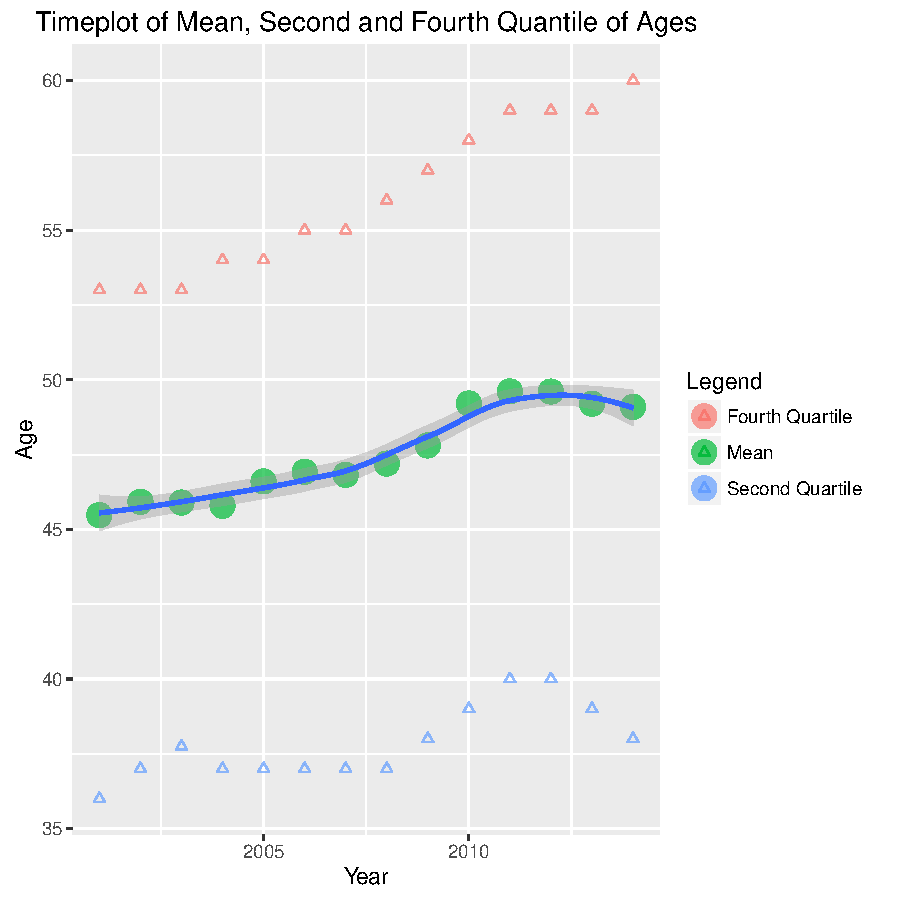
\includegraphics{facage-007}
\begin{Schunk}
\begin{Sinput}
> statsummary("histogram")
\end{Sinput}
\end{Schunk}
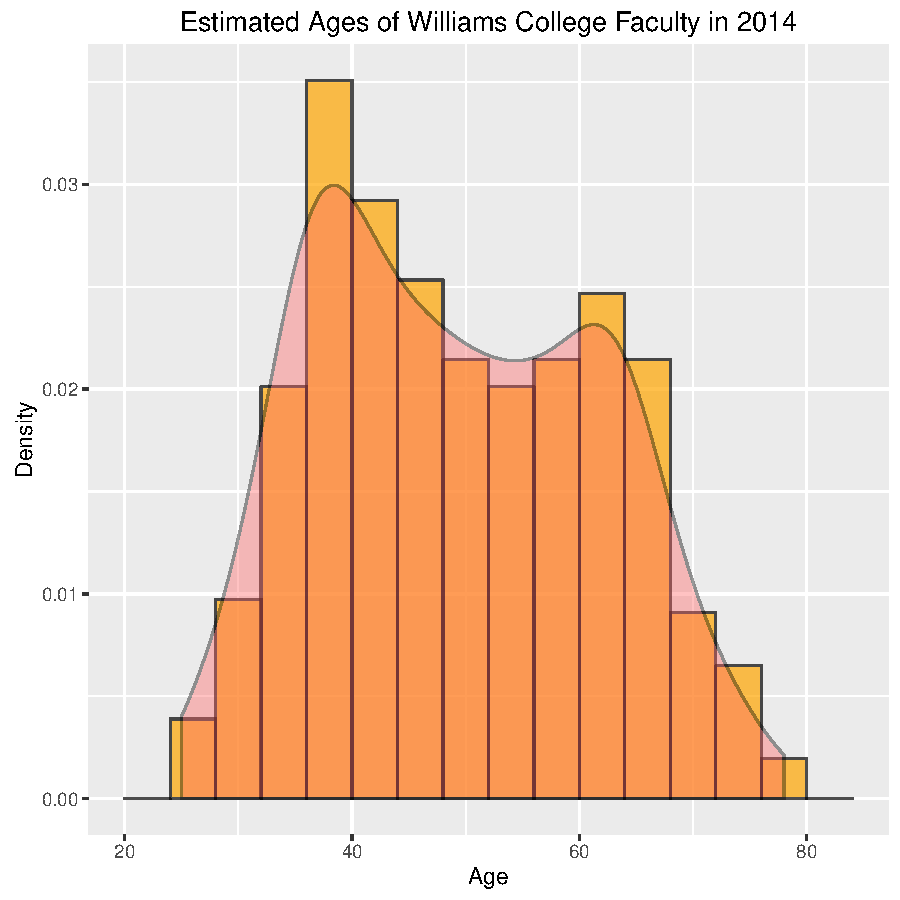
\includegraphics{facage-008}
\begin{Schunk}
\begin{Sinput}
> statsummary("comparison")
\end{Sinput}
\end{Schunk}
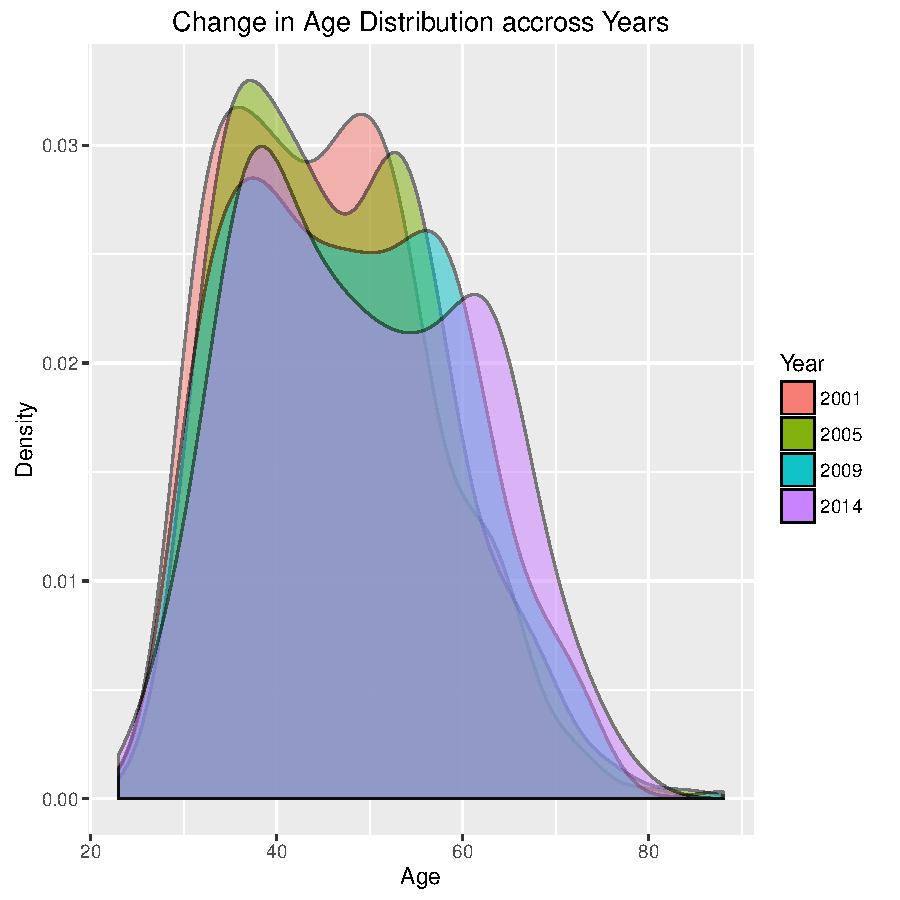
\includegraphics{facage-009}

\section{Conclusion}
The summary statistics indicate that the estimated average age of professors in 2014 was 49.1 years. The range of ages was 53 years with the minimum at 25 and maximum at 78. The graphics produced above yield some interesting results that might be worth noting. It is clearly seen from the timeplot and comparison plot that the histogram is getting wider as time progresses. Thus the variation in the ages of faculty within a given year is increasing, which is also indicated in the increase in standard deviation over time. There also seems to be trend in which the average age of the faculty is increasing. It is hard to tell whether this is due to an internal bias or due to the dynamics of a population structure. There is yet another intriguing observation. The age distribution seems to form two peaks which have persisted accross the years. The first peak is around 37 years and has stayed constant for 14 years, but the second peak has moved from 50 years in 2001 to 65 years in 2014. Again, the reason for this is not very evident and cannot be isolated without additional information.

The package \code{facage} includes functions that allow easy reading and analysis of data published by Williams College. This allows the study of the age distribution of professors at the college to be done in a very user friendly manner. That said, there is a lot of scope for future improvements to the package. The next big step in its development would be the ability to scan information about the department of the professors. This would allow the study of how the size and composition of departments at Williams have been changing over time. It might also allow for predictive ability of how particular departments might perform in the future.
There is further scope of modelling the dynamics of how the age distribution changes over time depending on what is the average rate of induction and retirement. These values could be estimated by running simulations on the currently existing data and might give insights about the pattern of hiring in relation with age accross departments.

\address{Arjun Kakkar\\
  Mathematics\\
  Williams College\\
  Williamstown, MA, USA\\}
\email{ak23@williams.edu}

\end{article}

\end{document}




